\documentclass[journal]{IEEEtran}
\usepackage[utf8]{inputenc}
\usepackage[spanish]{babel}
\usepackage{amsmath}
\usepackage{amsfonts}
\usepackage{amssymb}
\usepackage{graphicx}
\author{Cesar Cardozo}
\title{Algoritmo PSO aplicado a Busqueda y Rescate con Drones}
\begin{document}
\maketitle
\begin{abstract}
El presente articulo busca brindar una solución eficiente y efectiva para el apoyo en labores de busqueda y rescate en lugares de dificil recorrido. Esto haciendo uso de un ``Enjambre de Drones'' controlados mediante algoritmos comportamentales de PSO que resulten en una alternatia mucho más economica que los protocolos de rescate actualmente usados.\\

Así pues el principal objetivo es optimizar los gastos economicos que las instituciones deberían de hacer para llevar a cabo rescates de personas perdidas en cualquier tipo de terreno, ademas de disminuir tambien el tiempo de busqueda mediante esfuerzos combinados de hombre-maquina aumentando así las probabilidades de supervivencia de las personas perdidas.
\end{abstract}
\section{Introducción}
Según el ministerio de ambiente de Colombia, la cantidad creciente de personas (residentes y extranjeras) que acuden a los parques nacionales del país desde el 2015 ha causado, como es de suponer, un aumento proporcional en la cantidad de personas que se extravían en los territorios de los mismos; por esta razón el Minambiente ha obligado a los turistas a adquirir polizas de seguro que cubran los gastos de los protocolos establecidos para busqueday rescate.\\

Los costos de los rescates varian de la complejidad geografica, la cantidad de personas perdidas, las condiciones climatologicas y varios factores más que hacen imposibe estimar un presupuesto previo al rescate. Estos factores tambien afectan directamente el tiempo que se deba emplear en la busqueda de los individuos.\\

Actualmente se emplean metodologias de busqueda especializadas que mezclan componentes empiricos y teoricos con el fin de optimizar el rendimiento de los protocolos de busqueda y rescate, sin embargo se estan comenzando a implementar nuevas tecnologias que aceleren el proceso, por ejemplo naves no tripuladas.\\

\section{Metodos tipicos de Busqueda y Rescate}
\subsection{Caracterización}
El primer paso para llevar a cabo un rescate efectivo es la caracterización de el personal que se extravio, así como la zona en la que sucedio, con el fin de abstraer ciertos comportamientos que resultarán en delimitaciones y priorizaciones de las areas de busqueda.\\

Uno de los criterios a tener en cuenta es la edad de la persona extraviada, dado que sus condiciones psicologicas en general, aumentan o disminuyen las probabilidades de encontrarles en ciertos tipos de lugares.\\

Para los niños entre 4 y 6 años en su etapa preoperatoria ya se entienden las relaciones de causa y efecto, por lo que su tendencia es la de ir por sennderos y cominos, sin embargo de llegar a alterarse pueden desorientarse y alejarse de dichos puntos .\\

Para los niños entre 7 a 12 años dada su capacidad de orientación mayor, les resulta más facil conservar la calma, orientarse y volver de regreso al punto de partida (ULC).\\

En la edad entre 13 a 17 años el niño tendera a moverse a zonas en donde pueda adquirir mayor información para tomar decisiones a cerca de donde moverse, p.e. lugares altos o poblados.\\

Para un adulto, debido a que la causa más probable de perdida sea la de tomar un camino por error, la confianza en su propia cognición y su incapacidad de admitir equivocaiones hacen que el individuo se aleje mas del ULC.\\

\begin{center}
\begin{figure}
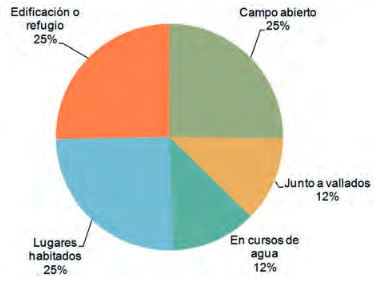
\includegraphics[width=0.4\textwidth]{4a6}
\textbf{\caption{``Probabilidad de localización niños entre 4 a 6 Años''}}
\end{figure}
\end{center}

\begin{center}
\begin{figure}
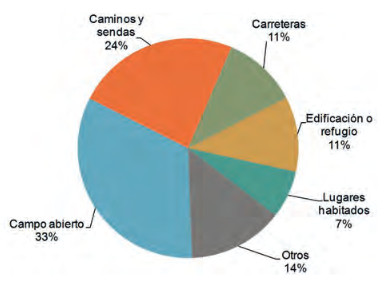
\includegraphics[width=0.4\textwidth]{7a12}
\textbf{\caption{``Probabilidad de localización niños entre 7 a 12 Años''}}
\end{figure}
\end{center}

\begin{center}
\begin{figure}
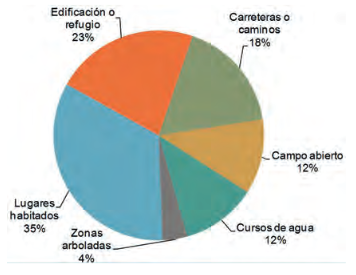
\includegraphics[width=0.4\textwidth]{13a17}
\textbf{\caption{``Probabilidad de localización niños entre 13 a 17 Años''}}
\end{figure}
\end{center}

\begin{center}
\begin{figure}
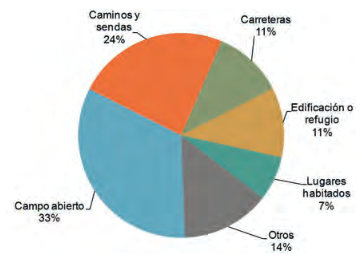
\includegraphics[width=0.4\textwidth]{18oMas}
\textbf{\caption{``Probabilidad de localización adultos mayores a 18 Años''}}
\end{figure}
\end{center}

\subsection{ULC y radio de busqueda}
El primer acercamiento que se realiza tras la carecterización es el Ultimo Lugar Conicido (ULC) de la persona perdida, a partir de este y con criterios preestablecidos según la condicion fisic y psicologica del individuo se determina un radio a traves del que la persona pudo haberse desplazado en linea recta independientemente de la geologia del terreno.

\begin{center}
\begin{figure}[h]
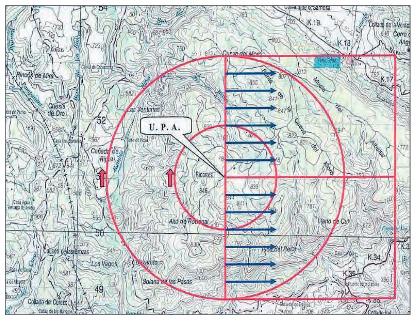
\includegraphics[width=0.4\textwidth]{Radio_SnR}
%\textbf{\caption{``Areas de busqueda determinadas por el ULC y los radios dependientes.''}}
\end{figure}
\end{center}

Se sobreentiende que este metodo es meramente empirico y que las areas que se obtienen aumentan de manera exponencial conforme pasa el tiempo dificultando la busqueda de una manera gradual.

\subsection{Busquedas con Drones}
Actualmente la busqueda de grandes areas con drones se lleva a cabo de manera mecanica y predefinida, los drones patrullan en la manera que se dispongan en el programa, de manera paralela con camaras de calor o de alta definición y enviando las señales captadas a la central para un análisis manual.

Al contrario de los excesivos costos de un rescate con vehiculos aereos tripulados, que se encuentran sobre los 4000 euros o 15 millones de pesos colombianos (tan solo el despliegue), la comodidad de transporte y despegue de los drones ademas de funcionar con batería los hacen extremadamente economicos para este proposito, y por ende una opción tentativa muy viable. 
\section{PSO en busqueda y rescate}
\subsection{Algoritmo PSO}
\textit{Particle Swamp Optimization} por sus siglas en ingles, es un algoritmo que se basa en el movimiento de las particulas sobre un plano y su comunicación para encontrar optimos locales y compararlo con los encontrados por otros componentes del enjambre para así llegar a una notable aproximación del optimo global.


\end{document}